%%%%%%%%%%%%%%%%%%%%%%%%%%%%%%%%%%%%%%%%%%%%%%%%%%%%%%%%%%%%%%%%%%%
% Method
% Team:
% Union
% Members: 
% Bernie Huang, Jim Lan, Hoang Tan, Kenny Hsu, Rahul Aditya, Tan Phat, Wei
% Relative files:
% Method_Union.tex
% Note:    
% Do not compile this file compile Main.tex to get the pdf file instead.
%%%%%%%%%%%%%%%%%%%%%%%%%%%%%%%%%%%%%%%%%%%%%%%%%%%%%%%%%%%%%%%%%%%
	
\subsection*{Title extraction}

\subsubsection*{Author abstraction}
\begin{itemize}
	\item I use the python to catch the abstract.
	\begin{center}
		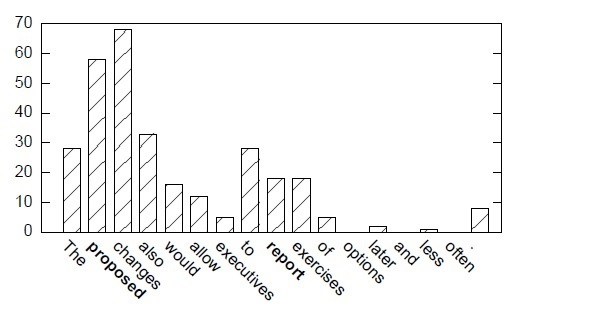
\includegraphics[width=0.8\columnwidth]{Union_Background_Chart_2}
	\end{center}
	\item Fist,the pdf be converted into txt.So it will create the txt file.\\ 
	\item Fist,the pdf be converted into txt.So it will create the txt file.\\ 	
	(a) Word Count $>$ 15\\
	(b) 15 $>$ Word Count $>$ 10\\
	(c) 10 $>$ Word Count $>$5\\
	(d) 5 $>$Word Count	
	\begin{center}
		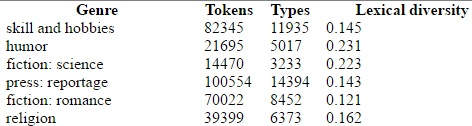
\includegraphics[width=0.8\columnwidth]{Union_Background_Chart_3}
	\end{center}
	\item search : Search Word repetition rate
	\item statistics: Count the repetition rate of words
	\item sort: Show the number of rankings
\end{itemize}

\subsubsection*{Abstract extraction}

\nwepage
